\documentclass[12pt,letterpaper]{exam}
\usepackage[lmargin=1in,rmargin=1in,tmargin=1in,bmargin=1in]{geometry}
\usepackage{../style/exams}

% -------------------
% Course & Exam Information
% -------------------
\newcommand{\course}{MATH 142: Final Exam}
\newcommand{\term}{Spring --- 2025}
\newcommand{\examdate}{05/06/2025}
\newcommand{\timelimit}{150 Minutes}

\setbool{hideans}{true} % Student: True; Instructor: False
% For this exam, if false, uncomment \renewcommand{\tikzmark} below

\newcommand{\boxseven}[4]{%
	\draw[thick] (0,0) -- (4,0) -- (4,4) -- (0,4) -- (0,0);
	\draw[thick] (0,2) -- (4,2);
	\draw[thick] (2,0) -- (2,4);
	% '7'
	\draw (1.7,2.2) -- (2.3,2.2) -- (1.7,1.6);
	% Entries
	\node at (1,3) {$#1$};	% u
	\node at (3,1) {$#2$};	% dv
	\node at (1,1) {$#3$};	% du
	\node at (3,3) {$#4$};	% 
}


\usetikzlibrary{calc}
\usepackage{booktabs}
\tikzset{Arrow Style/.style={text=black, font=\boldmath}}
%\renewcommand{\tikzmark}[1]{%
%    \tikz[overlay, remember picture, baseline] \node (#1) {};%
%}
\newcommand*{\XShift}{0.5em}
\newcommand*{\YShift}{0.5ex}
\NewDocumentCommand{\DrawArrow}{s O{} m m m}{%
    \begin{tikzpicture}[overlay,remember picture]
        \draw[->, thick, Arrow Style, #2] 
                ($(#3.west)+(\XShift,\YShift)$) -- 
                ($(#4.east)+(-\XShift,\YShift)$)
        node [midway,above] {#5};
    \end{tikzpicture}%
}
\usepackage{cancel}

\usepgfplotslibrary{fillbetween}
\usepackage{relsize}

% -------------------
% Content
% -------------------
\begin{document}

\examtitle
\instructions{Write your name on the appropriate line on the exam cover sheet. This exam contains \numpages\ pages (including this cover page) and \numquestions\ questions. Check that you have every page of the exam. \pspace

This exam consists of three parts---each corresponding to a previous course exam---with six questions. {\bfseries Choose 5 of the 6 questions for each part and answer only these 5 questions.} That is, choose five of the six questions from Questions~1 through 6, choose five of the six questions from Questions 7 through 12, and choose five of the six questions from Questions 13 through 18 to answer and answer only these questions. Clearly indicate which questions you are choosing \textit{not} to answer by crossing out their score box on the cover page. You are not required to answer the bonus questions and doing so will not adversely affect your score. \pspace


Answer the questions in the spaces provided on the question sheets. Be sure to answer every part of each chosen question and show all your work. If you run out of room for an answer, continue on the back of the page --- being sure to indicate the problem number.} 

%\scores
{\renewcommand{\arraystretch}{1.8}
	\begin{table}[!ht]
	\centering
	\begin{tabular}{ccccccccc} \hline \rowcolor[HTML]{C0C0C0} 
	\multicolumn{3}{|c|}{\cellcolor[HTML]{C0C0C0}\textbf{Exam 1}} & \multicolumn{3}{c|}{\cellcolor[HTML]{C0C0C0}\textbf{Exam 2}} & \multicolumn{3}{c|}{\cellcolor[HTML]{C0C0C0}\textbf{Exam 3}} \\ \hline
\rowcolor[HTML]{C0C0C0} 
	
	\multicolumn{1}{|c|}{\cellcolor[HTML]{C0C0C0}Question} & \multicolumn{1}{c|}{\cellcolor[HTML]{C0C0C0}Points} & \multicolumn{1}{c|}{\cellcolor[HTML]{C0C0C0}Score} & \multicolumn{1}{c|}{\cellcolor[HTML]{C0C0C0}Question} & \multicolumn{1}{c|}{\cellcolor[HTML]{C0C0C0}Points} & \multicolumn{1}{c|}{\cellcolor[HTML]{C0C0C0}Score} & \multicolumn{1}{c|}{\cellcolor[HTML]{C0C0C0}Question} & \multicolumn{1}{c|}{\cellcolor[HTML]{C0C0C0}Points} & \multicolumn{1}{c|}{\cellcolor[HTML]{C0C0C0}Score} \\ \hline

	\multicolumn{1}{|c|}{\cellcolor[HTML]{C0C0C0}1} & \multicolumn{1}{c|}{10} & \multicolumn{1}{c|}{} & \multicolumn{1}{c|}{\cellcolor[HTML]{C0C0C0}7} & \multicolumn{1}{c|}{10} & \multicolumn{1}{c|}{} & \multicolumn{1}{c|}{\cellcolor[HTML]{C0C0C0}13} & \multicolumn{1}{c|}{10} & \multicolumn{1}{c|}{} \\ \hline

	\multicolumn{1}{|c|}{\cellcolor[HTML]{C0C0C0}2} & \multicolumn{1}{c|}{10} & \multicolumn{1}{c|}{} & \multicolumn{1}{c|}{\cellcolor[HTML]{C0C0C0}8} & \multicolumn{1}{c|}{10} & \multicolumn{1}{c|}{} & \multicolumn{1}{c|}{\cellcolor[HTML]{C0C0C0}14} & \multicolumn{1}{c|}{10} & \multicolumn{1}{c|}{} \\ \hline
	
	\multicolumn{1}{|c|}{\cellcolor[HTML]{C0C0C0}3} & \multicolumn{1}{c|}{10} & \multicolumn{1}{c|}{} & \multicolumn{1}{c|}{\cellcolor[HTML]{C0C0C0}9} & \multicolumn{1}{c|}{10} & \multicolumn{1}{c|}{} & \multicolumn{1}{c|}{\cellcolor[HTML]{C0C0C0}15} & \multicolumn{1}{c|}{10} & \multicolumn{1}{c|}{} \\ \hline

	\multicolumn{1}{|c|}{\cellcolor[HTML]{C0C0C0}4} & \multicolumn{1}{c|}{10} & \multicolumn{1}{c|}{} & \multicolumn{1}{c|}{\cellcolor[HTML]{C0C0C0}10} & \multicolumn{1}{c|}{10} & \multicolumn{1}{c|}{} & \multicolumn{1}{c|}{\cellcolor[HTML]{C0C0C0}16} & \multicolumn{1}{c|}{10} & \multicolumn{1}{c|}{} \\ \hline

	\multicolumn{1}{|c|}{\cellcolor[HTML]{C0C0C0}5} & \multicolumn{1}{c|}{10} & \multicolumn{1}{c|}{} & \multicolumn{1}{c|}{\cellcolor[HTML]{C0C0C0}11} & \multicolumn{1}{c|}{10} & \multicolumn{1}{c|}{} & \multicolumn{1}{c|}{\cellcolor[HTML]{C0C0C0}17} & \multicolumn{1}{c|}{10} & \multicolumn{1}{c|}{} \\ \hline

	\multicolumn{1}{|c|}{\cellcolor[HTML]{C0C0C0}6} & \multicolumn{1}{c|}{10} & \multicolumn{1}{c|}{} & \multicolumn{1}{c|}{\cellcolor[HTML]{C0C0C0}12} & \multicolumn{1}{c|}{10} & \multicolumn{1}{c|}{} & \multicolumn{1}{c|}{\cellcolor[HTML]{C0C0C0}18} & \multicolumn{1}{c|}{10} & \multicolumn{1}{c|}{} \\ \hline

	\multicolumn{1}{|c|}{\cellcolor[HTML]{C0C0C0}\textbf{Total}} & \multicolumn{1}{c|}{50} & \multicolumn{1}{c|}{} & \multicolumn{1}{c|}{\cellcolor[HTML]{C0C0C0}\textbf{Total}} & \multicolumn{1}{c|}{50} & \multicolumn{1}{c|}{} & \multicolumn{1}{c|}{\cellcolor[HTML]{C0C0C0}\textbf{Total}} & \multicolumn{1}{c|}{50} & \multicolumn{1}{c|}{} \\[0.2cm] \hline

&  &  & {\bfseries Exam Total:} & &  &  &  & 
\end{tabular}
\end{table}
}
\bottomline
\newpage


% -------------------
% Questions
% -------------------
\begin{questions}

% Question 1
\newpage
\question[10] Showing all your work, evaluate the following:
	\[
	\int x^3 \ln x \;dx
	\] \pspace

\sol{We integrate this using integration-by-parts. Using LIATE, we choose $u= \ln x$, which forces $dv= x^3$. But then we have\dots
	\[
	\begin{tikzpicture}
	\boxseven{\ln x}{x^3}{\dfrac{1}{x}}{\dfrac{1}{4}\, x^4}
	\end{tikzpicture}
	\]
That is, $du= \frac{1}{x} \, dx$ and $v= \frac{1}{4} \, x^4$. Therefore, we have\dots
	\[
	\begin{aligned}
	\int x^3 \ln x \;dx&= \dfrac{1}{4} \, x^4 \ln x - \int \dfrac{1}{4} \, x^3 \;dx \\[0.3cm]
	&= \dfrac{1}{4} \, x^4 \ln x - \dfrac{1}{4} \int x^3 \;dx \\[0.3cm]
	&= \dfrac{1}{4} \, x^4 \ln x - \dfrac{1}{4} \cdot \dfrac{x^4}{4} + C \\[0.3cm]
	&= \boxed{\dfrac{1}{4} \, x^4 \ln x - \dfrac{x^4}{16} + C} \\[0.3cm]
	&= \dfrac{x^4}{16} \left( 4 \ln x - 1 \right) + C
	\end{aligned}
	\]
}



% Question 2
\newpage
\question[10] Showing all your work, compute the following:
	\[
	\int \dfrac{x^2}{\sqrt{9 - x^2}} \;dx
	\] \pspace

\sol{We know from the Pythagorean Theorem that $a^2 + b^2= c^2$, which implies that $a^2= c^2 - b^2$. Taking $c^2= 9$, i.e. $c= 3$, and $b^2= x^2$, i.e. $b= x$, we have $a^2= c^2 - b^2= 9 - x^2$. This also shows that $a= \sqrt{9 - x^2}$. There are two possible right triangles corresponding to these sides we could draw:
	\[
	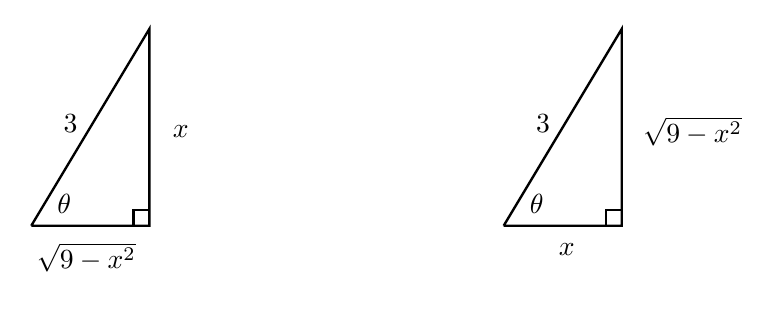
\begin{tikzpicture}
	\draw[line width=0.03cm] (0,0) -- (1.5,0) -- (1.5,2.5) -- (0,0);
	\draw[line width=0.03cm] (1.3,0) -- (1.3,0.2) -- (1.5,0.2);
	\node at (0.7,-0.4) {$\sqrt{9 - x^2}$};
	\node at (1.9,1.2) {$x$};
	\node at (0.5,1.3) {$3$};
	\node at (0.42,0.28) {$\theta$};
	
	\tikzset{shift={(6,0)}};

	\draw[line width=0.03cm] (0,0) -- (1.5,0) -- (1.5,2.5) -- (0,0);
	\draw[line width=0.03cm] (1.3,0) -- (1.3,0.2) -- (1.5,0.2);
	\node at (0.8,-0.3) {$x$};
	\node at (2.4,1.2) {$\sqrt{9 - x^2}$};
	\node at (0.5,1.3) {$3$};
	\node at (0.42,0.28) {$\theta$};
	\end{tikzpicture}
	\] \par
Using the triangle on the left, we have $\sin \theta= \frac{x}{3}$, which implies $x= 3 \sin \theta$. [This also means $x^2= (3 \sin \theta)^2= 9 \sin^2 \theta$.] But then $dx= 3 \cos \theta \;d\theta$. We also know that $\cos \theta= \frac{\sqrt{9 - x^2}}{3}$, so that $\sqrt{9 - x^2}= 3 \cos \theta$. Therefore, we have\dots
	\[
	\int \dfrac{x^2}{\sqrt{9 - x^2}} \;dx= \int \dfrac{9 \sin^2 \theta}{3 \cos \theta} \cdot 3 \cos \theta \;d\theta= 9 \int \sin^2 \theta \;d\theta
	\]
Using the fact that $\sin^2 \theta= \frac{1 - \cos(2\theta)}{2}$, we have\dots
	\[
	9 \int \sin^2 \theta \;d\theta= 9 \int \dfrac{1 - \cos(2\theta)}{2} \;d\theta= \dfrac{9}{2} \int 1 - \cos 2 \theta \;d\theta= \dfrac{9}{2} \left( \theta - \dfrac{\sin 2 \theta}{2} \right) + C
	\]
We know that $\sin(2 \theta)= 2 \sin \theta \cos \theta$, which implies\dots 
	\[
	\dfrac{9}{2} \left( \theta - \dfrac{\sin 2 \theta}{2} \right) + C= \dfrac{9}{2} \left( \theta - \dfrac{2 \sin \theta \cos \theta}{2} \right) + C= \dfrac{9}{2} \left( \theta - \sin \theta \cos \theta \right) + C
	\]

Using the triangle on the left above, we know that $\sin \theta= \frac{x}{3}$ and $\cos \theta= \frac{\sqrt{9 - x^2}}{3}$. We also know that $x= 3 \sin \theta$, which implies that $\sin \theta= \frac{x}{3}$ and $\theta= \sin^{-1} \left( \frac{x}{3} \right)$. Therefore, we know\dots
	\[
	\hspace{-0.5cm} \dfrac{9}{2} \left( \theta - \sin \theta \cos \theta \right) + C= \dfrac{9}{2} \left( \sin^{-1} \left( \dfrac{x}{3} \right) - \dfrac{x}{3} \cdot \dfrac{\sqrt{9 - x^2}}{3} \right) + C= \dfrac{9}{2} \left( \sin^{-1} \left( \dfrac{x}{3} \right) - \dfrac{x \sqrt{9 - x^2}}{9} \right) + C
	\]
But then, we know\dots
	\[
	\int \dfrac{x^2}{\sqrt{9 - x^2}} \;dx= \boxed{\dfrac{9}{2} \left( \sin^{-1} \left( \dfrac{x}{3} \right) - \dfrac{x \sqrt{9 - x^2}}{9} \right) + C}=  \dfrac{1}{2} \left( 9 \sin^{-1} \left( \dfrac{x}{3} \right) - x \sqrt{9 - x^2} \right) + C
	\]
}

\remove{\newpage

\sol{%
\thispagestyle{empty} \newline
\noindent Using the triangle on the left, we have $\sin \theta= \frac{x}{3}$, which implies $x= 3 \sin \theta$. [This also means $x^2= (3 \sin \theta)^2= 9 \sin^2 \theta$.] But then $dx= 3 \cos \theta \;d\theta$. We also know that $\cos \theta= \frac{\sqrt{9 - x^2}}{3}$, so that $\sqrt{9 - x^2}= 3 \cos \theta$. Therefore, we have\dots
	\[
	\int \dfrac{x^2}{\sqrt{9 - x^2}} \;dx= \int \dfrac{9 \sin^2 \theta}{3 \cos \theta} \cdot 3 \cos \theta \;d\theta= 9 \int \sin^2 \theta \;d\theta
	\]
Using the fact that $\sin^2 \theta= \frac{1 - \cos(2\theta)}{2}$, we have\dots
	\[
	9 \int \sin^2 \theta \;d\theta= 9 \int \dfrac{1 - \cos(2\theta)}{2} \;d\theta= \dfrac{9}{2} \int 1 - \cos 2 \theta \;d\theta= \dfrac{9}{2} \left( \theta - \dfrac{\sin 2 \theta}{2} \right) + C
	\]
We know that $\sin(2 \theta)= 2 \sin \theta \cos \theta$, which implies\dots 
	\[
	\dfrac{9}{2} \left( \theta - \dfrac{\sin 2 \theta}{2} \right) + C= \dfrac{9}{2} \left( \theta - \dfrac{2 \sin \theta \cos \theta}{2} \right) + C= \dfrac{9}{2} \left( \theta - \sin \theta \cos \theta \right) + C
	\]

Using the triangle on the left above, we know that $\sin \theta= \frac{x}{3}$ and $\cos \theta= \frac{\sqrt{9 - x^2}}{3}$. We also know that $x= 3 \sin \theta$, which implies that $\sin \theta= \frac{x}{3}$ and $\theta= \sin^{-1} \left( \frac{x}{3} \right)$. Therefore, we know\dots
	\[
	\dfrac{9}{2} \left( \theta - \sin \theta \cos \theta \right) + C= \dfrac{9}{2} \left( \sin^{-1} \left( \dfrac{x}{3} \right) - \dfrac{x}{3} \cdot \dfrac{\sqrt{9 - x^2}}{3} \right) + C= \dfrac{9}{2} \left( \sin^{-1} \left( \dfrac{x}{3} \right) - \dfrac{x \sqrt{9 - x^2}}{9} \right) + C
	\]
But then, we know\dots
	\[
	\int \dfrac{x^2}{\sqrt{9 - x^2}} \;dx= \boxed{\dfrac{9}{2} \left( \sin^{-1} \left( \dfrac{x}{3} \right) - \dfrac{x \sqrt{9 - x^2}}{9} \right) + C}=  \dfrac{1}{2} \left( 9 \sin^{-1} \left( \dfrac{x}{3} \right) - x \sqrt{9 - x^2} \right) + C
	\]
   }
}



% Question 3
\newpage
\question[10] Showing all your work, evaluate the following:
	\[
	\int_0^\pi \sin^3 \theta \cos^2 \theta \;d\theta
	\]

\sol{We can replace even powers of $\sin \theta$ or $\cos \theta$ using the identity $\sin^2 \theta + \cos^2 \theta= 1$. If $u= \sin \theta$, the `$du$ factor' removes one power of $\cos \theta$ in the integrand leaving a single power of $\cos \theta$ that cannot be replaced. Therefore, we must choose $u= \cos \theta$. This implies that $du= -\sin \theta \;d\theta$. If $\theta= \pi$, then $u= \cos(\pi)= -1$. If $\theta= 0$, then $u= \cos(0)= 1$. Using the identity $\sin^2 \theta + \cos^2 \theta= 1$, we know that $\sin^2 \theta= 1 - \cos^2 \theta$. Therefore, we have\dots
	\[
	\begin{aligned}
	\int_0^\pi \sin^3 \theta \cos^2 \theta \;d\theta&= \int_0^\pi (\sin^2 \theta \cos^2 \theta) \cdot \sin \theta \; d\theta \\
	&= -\int_0^\pi (\sin^2 \theta \cos^2 \theta) \cdot (-\sin \theta) \; d\theta \\[0.3cm]
	&= -\int_0^\pi \big( (1 - \cos^2 \theta) \cos^2 \theta \big) \cdot (-\sin \theta) \; d\theta \\[0.3cm]
	&= -\int_1^{-1} (1 - u^2) u^2 \;du \\[0.3cm]
	&= \int_{-1}^1 (1 - u^2) u^2 \;du \\[0.3cm]
	&= \int_{-1}^1 (u^2 - u^4) \;du \\[0.3cm]
	&= \dfrac{u^3}{3} - \dfrac{u^5}{5} \bigg|_{-1}^1 \\[0.3cm]
	&= \left( \dfrac{1}{3} - \dfrac{1}{5} \right) - \left( \dfrac{(-1)^3}{3} - \dfrac{(-1)^5}{5} \right) \\[0.3cm]
	&= \left( \dfrac{1}{3} - \dfrac{1}{5} \right) - \left( \dfrac{-1}{3} - \dfrac{-1}{5} \right) \\[0.3cm]
	&= \dfrac{1}{3} - \dfrac{1}{5} + \dfrac{1}{3} + \dfrac{-1}{5} \\[0.3cm]
	&= \dfrac{2}{3} - \dfrac{2}{5} \\[0.3cm]
	&= \dfrac{10}{15} - \dfrac{6}{15} \\[0.3cm]
	&= \boxed{\dfrac{4}{15}}
	\end{aligned}
	\]
}



% Question 4
\newpage
\question[10] Showing all your work, evaluate the following integral:
	\[
	\int \dfrac{x^2 + 11x + 3}{(x - 1)^2 (x + 4)} \;dx
	\]

\sol{We use partial fractions. Observe the integrand can be decomposed as\dots
	\[
	\dfrac{x^2 + 11x + 3}{(x - 1)^2 (x + 4)}= \dfrac{A}{x - 1} + \dfrac{B}{(x - 1)^2} + \dfrac{C}{x + 4}
	\]
Using Heaviside's method, we can immediately determine $B$ and $C$. The `bad' number associated to $B$ is $x= 1$, while the `bad' number associated to $C$ is $x= -4$. Using these, we find\dots
	\[
	\begin{aligned}
	B&= \dfrac{x^2 + 11x + 3}{x + 4} \bigg|_{x=1}= \dfrac{1 + 11 + 3}{1 + 4}= \dfrac{15}{5}= 3 \\[0.3cm]
	C&= \dfrac{x^2 + 11x + 3}{(x - 1)^2} \bigg|_{x= -4}= \dfrac{16 - 44 + 3}{(-5)^2}= \dfrac{-25}{25}= -1
	\end{aligned}
	\]
To determine $A$, we can use any $x$-value with $x \neq -4, 1$. Using $x= 0$, we know\dots
	\[
	\begin{gathered}
	\dfrac{x^2 + 11x + 3}{(x - 1)^2 (x + 4)}= \dfrac{A}{x - 1} + \dfrac{B}{(x - 1)^2} + \dfrac{C}{x + 4} \\
	\dfrac{0 + 0 + 3}{(-1)^2 \cdot 4}= \dfrac{A}{0 - 1} + \dfrac{3}{(-1)^2} + \dfrac{-1}{4} \\
	\dfrac{3}{4}= -A + 3 - \dfrac{1}{4} \\
	3= -4A + 12 - 1 \\
	-8= -4A \\
	A= 2
	\end{gathered}
	\]
Alternatively, one could have found a common denominator---namely $(x - 1)^2(x + 4)$---on both sides of the equality above. Equating numerators, one would have $x^2 + 11x + 3= A(x - 1)(x + 4) + B(x + 4) + C(x - 1)^2$. Equating coefficients, this leads to the system of equations $A + C= 1$, $3A + B - 2C= 11$, and $-4A + 4B + C= 3$. Therefore, we have\dots
	\[
	\begin{aligned}
	\int \dfrac{x^2 + 11x + 3}{(x - 1)^2 (x + 4)} \;dx&= \int \dfrac{2}{x - 1} + \dfrac{3}{(x - 1)^2} + \dfrac{-1}{x + 4} \;dx \\[0.3cm]
	&= \boxed{2 \ln|x - 1| - \dfrac{3}{x - 1} - \ln|x + 4| + K}
	\end{aligned}
	\]
}



% Question 5
\newpage
\question[10] Determine whether the following improper integral converges or diverges. If it converges, compute the value of the integral. Be sure to rigorously justify all your computations. 
	\[
	\int_2^\infty \dfrac{dx}{x \, (\ln x)^2}
	\] \pspace

\sol{We first find the indefinite integral. Let $u= \ln x$ so that $du= \dfrac{1}{x} \, \;dx$. But then we have\dots
	\[
	\int \dfrac{dx}{x (\ln x)^2}= \int \dfrac{1}{(\ln x)^2} \cdot \dfrac{1}{x} \;dx= \int \dfrac{1}{u^2} \;du= -\dfrac{1}{u} + C= -\dfrac{1}{\ln x} + C
	\]
Therefore, we have\dots
	\[
	\begin{aligned}
	\int_2^\infty \dfrac{dx}{x \, (\ln x)^2}&= \lim_{b \to \infty} \int_2^b \dfrac{dx}{x \, (\ln x)^2} \\[0.3cm]
	&= \lim_{b \to \infty} -\dfrac{1}{\ln x} \bigg|_2^b \\[0.3cm]
	&= \lim_{b \to \infty} -\dfrac{1}{\ln b} - \dfrac{-1}{\ln 2} \\[0.3cm]
	&= 0 + \dfrac{1}{\ln 2} \\[0.3cm]
	&= \boxed{\dfrac{1}{\ln 2}}
	\end{aligned}
	\]
}



% Question 6
\newpage
\question[10] Showing all your work, find the following:
	\[
	\int x^2 \sin(2x) \;dx
	\] \pspace

\remove{%
\sol{We use tabular integration. Choosing $u= x^2$ and $dv= \sin(2x)$, we have\dots
	\[
	\begin{array}{c @{\hspace*{1.3cm}} c} \toprule
	u & dv \\ \cmidrule(lr){1-2}
	x^2 \tikzmark{Left 1} & \tikzmark{Right 1} \sin(2x) \\[0.3cm]
	2x \tikzmark{Left 2} & \tikzmark{Right 2} -\dfrac{1}{2} \, \cos(2x) \\[0.3cm]
	2 \tikzmark{Left 3} & \tikzmark{Right 3} -\dfrac{1}{4} \, \sin(2x) \\[0.3cm]
	0 \tikzmark{Left 4} & \tikzmark{Right 4} \dfrac{1}{8} \, \cos(2x) \\[0.3cm]
	
	\DrawArrow{Left 1}{Right 2}{+}
	\DrawArrow{Left 2}{Right 3}{--}
	\DrawArrow{Left 3}{Right 4}{+}
	\end{array}
	\]
Therefore, we have\dots
	\[
	\int x^2 \sin(2x) \;dx= \boxed{-\dfrac{1}{2} \, x^2 \cos(2x) + \dfrac{1}{2}\, x \sin(2x) + \dfrac{1}{4} \, \cos(2x) + C}
	\]
   }
}



% Question 7
\newpage
\question[10] Compute the arc length of the curve $y= 2+ 4x^{3/2}$, where $0 \leq x \leq 2$. \pspace

\sol{Recall that the arclength of a differentiable function $f(x)$ on an interval $[a, b]$ is given by\dots
	\[
	L= \int_a^b \sqrt{1 + \big( f'(x) \big)^2} \;dx
	\]
We have\dots
	\[
	\begin{aligned}
	f(x)&= 2 + 4 x^{3/2} \\[0.3cm]
	f'(x)&= 6x^{1/2}= 6 \sqrt{x} \\
	\\
	\big(f'(x) \big)^2&= (6 \sqrt{x})^2= 36 x
	\end{aligned}
	\] \pspace
Therefore, we have\dots 
	\[
	\begin{aligned}
	L&= \int_a^b \sqrt{1 + \big( f'(x) \big)^2} \;dx \\[0.3cm]
	&= \int_0^2 \sqrt{1 + 36x} \;dx \\[0.3cm]
	&= \dfrac{(1 + 36x)^{3/2}}{3/2} \cdot \dfrac{1}{36} \, \bigg|_0^2 \\[0.3cm]
	&= \dfrac{(1 + 36x)^{3/2}}{54} \bigg|_0^2 \\[0.3cm]
	&= \dfrac{1}{54} \left( (1 + 72)^{3/2} - (1 + 0)^{3/2} \right) \\[0.3cm]
	&= \boxed{\dfrac{1}{54} \left( 73^{3/2} - 1 \right)}
	\end{aligned}
	\]
}



% Question 8
\newpage
\question[10] Determine whether the following series is absolutely convergent, conditionally convergent, or divergent. Be sure to fully justify your reasoning with the appropriate series tests. 
	\[
	\sum_{n=0}^\infty (-1)^n \, \dfrac{n + 1}{n^2 + 1}
	\] \pspace

\sol{\relscale{0.78}{The given series is absolutely convergent, conditionally convergent, or divergent if and only if the series $\sum_{n=1}^\infty (-1)^n \, \dfrac{n + 1}{n^2 + 1}$ is as such. We then consider this latter series. Observe that this latter series is an alternating series. We know that\dots
	\begin{itemize}
	\item $\ds\lim_{n \to \infty} \dfrac{n + 1}{n^2 + 1}= 0$
	\item The sequence $\left\{ \dfrac{n + 1}{n^2 + 1} \right\}$ is decreasing for $n > 1$ (the first term does not affect whether the series converges or diverges).
	\end{itemize}
Therefore, by the Alternating Series Test, the series $\ds\sum_{n=1}^\infty (-1)^n \, \dfrac{n + 1}{n^2 + 1}$ converges. To determine whether the series is absolutely convergent, we need to determine whether the series $\ds\sum_{n=1}^\infty \dfrac{n + 1}{n^2 + 1}$ converges. \pspace

Observe that the series $\ds\sum_{n=1}^\infty \dfrac{1}{n}$ diverges by the $p$-test with $p= 1$. We know\dots
	\[
	\lim_{n \to \infty} \dfrac{\;\;\dfrac{n + 1}{n^2 + 1}\;\;}{\dfrac{1}{n}}= \lim_{n \to \infty} \dfrac{n^2 + n}{n^2 + 1}= 1
	\]
As this limit is finite and nonzero, we know that the series $\ds\sum_{n=1}^\infty \dfrac{n + 1}{n^2 + 1}$ diverges by the Limit Comparison Test. Alternatively, we know\dots
	\[
	\sum_{n=1}^\infty \dfrac{n + 1}{n^2 + 1} > \sum_{n=1}^\infty \dfrac{n}{n^2 + n^2}= \sum_{n=1}^\infty \dfrac{n}{2n^2}= \dfrac{1}{2} \sum_{n=1}^\infty \dfrac{1}{n}
	\]
Therefore, the series $\ds\sum_{n=1}^\infty \dfrac{n + 1}{n^2 + 1}$ diverges by the Direct Comparison Test. Alternatively, let $f(x)= \frac{x + 1}{x^2 + 1}$. This function is positive, decreasing, and continuous on $[1, \infty)$. We know that $\ds\int \frac{x + 1}{x^2 + 1} \;dx= \frac{1}{2} \, \ln|x^2 + 1| + C$. Therefore, we have\dots
	\[
	\int_1^\infty \dfrac{x + 1}{x^2 + 1} \;dx:= \lim_{b \to \infty} \int_1^b \dfrac{x + 1}{x^2 + 1} \;dx= \lim_{b \to \infty} \dfrac{1}{2} \ln|x^2 + 1| \;\bigg|_1^b= \lim_{b \to \infty} \dfrac{1}{2}\, \ln|b^2 + 1| - \dfrac{1}{2} \, \ln|2|= \infty
	\]
Because the integral diverges, $\ds\sum_{n=1}^\infty \dfrac{n + 1}{n^2 + 1}$ diverges by the Integral Test. \pspace

Because the series $\ds\sum_{n=0}^\infty (-1)^n \, \dfrac{n + 1}{n^2 + 1}$ converges and the series $\ds\sum_{n=1}^\infty \dfrac{n + 1}{n^2 + 1}$ diverges, we know that the series $\ds\sum_{n=0}^\infty (-1)^n \, \dfrac{n + 1}{n^2 + 1}$ is conditionally convergent.}}
	


% Question 9
\newpage
\question[10] Completely justifying your answer, determine whether the following series converges or diverges. If the series converges, compute its sum. 
	\[
	\sum_{n=1}^\infty \dfrac{3 (5^n)}{2^{3n}}
	\] \pspace

\sol{Observe that\dots
	\[
	\sum_{n=1}^\infty \dfrac{3 (5^n)}{2^{3n}}= \sum_{n=1}^\infty 3\,\dfrac{(5^n)}{(2^3)^n}= \sum_{n=1}^\infty \dfrac{3 (5^n)}{8^n}= \sum_{n=1}^\infty 3 \left( \dfrac{5}{8} \right)^n
	\]
This series is geometric, i.e. of the form $\ds\sum Ar^n$, with $A= 3$ and $r= \frac{5}{8}$. Because $|r|= \frac{5}{8} < 1$, this series converges by the Geometric Series Test. We know that the series converges to\dots
	\[
	\dfrac{\text{first term}}{1 - r}= \dfrac{\dfrac{3(5^1)}{2^3}}{1 - \dfrac{5}{8}}= \dfrac{\;\;\dfrac{15}{8}\;\;}{\dfrac{3}{8}}= \dfrac{\;\;\dfrac{15}{8}\;\;}{\dfrac{3}{8}} \cdot \dfrac{1/8}{1/8}= \dfrac{15}{3}= 5 
	\] \vfill

{\scriptsize Note. One can use any number of tests to determine that the series converges, but they will not allow one to find the sum. For instance, we have\dots
	\[
	\lim_{n \to \infty} \dfrac{\;\;\dfrac{3 (5^{n+1})}{2^{3(n+1)}}\;\;}{\dfrac{3 (5^n)}{2^{3n}}}= \lim_{n \to \infty} \dfrac{3 \cdot 5^{n + 1}}{2^{3n + 3}} \cdot \dfrac{2^{3n}}{3 \cdot 5^n}= \lim_{n \to \infty} \dfrac{3}{3} \cdot \dfrac{5^{n+1}}{5^n} \cdot \dfrac{2^{3n}}{2^{3n+3}}= \lim_{n \to \infty} \dfrac{5^n \,5}{5^n} \cdot \dfrac{2^{3n}}{2^{3n} \, 2^3}= \lim_{n \to \infty} \dfrac{5}{8}= \dfrac{5}{8}
	\]
Because $\frac{5}{8} < 1$, the series converges absolutely by the Ratio Test. \pspace

Alternatively, 
	\[
	\lim_{n \to \infty} \left( \dfrac{3(5^n)}{2^{3n}} \right)^{1/n}= \lim_{n \to \infty} \dfrac{3^{1/n} \, 5}{2^3}= \dfrac{1 \cdot 5}{8}= \dfrac{5}{8}
	\]
Because $\frac{5}{8} < 1$, the series converges absolutely by the Root Test. \pspace

Alternatively, using the representation of the summand on the right above, define $f(x)= 3 \left(\frac{5}{8}\right)^x$. Observe that $f(x)$ is positive, decreasing, and continuous on $[1, \infty)$. We know that $\ds\int 3 \left(\frac{5}{8}\right)^x \;dx= -\dfrac{3 (5/8)^x}{\ln(8/5)} + C$. Therefore, we have\dots
	\[
	\int_1^\infty 3 \left(\frac{5}{8}\right)^x \;dx:= \lim_{b \to \infty} \int_1^b 3 \left(\frac{5}{8}\right)^x \;dx= \lim_{b \to \infty} -\dfrac{3 (5/8)^x}{\ln(8/5)} \bigg|_1^b= \lim_{b \to \infty} -\dfrac{3 (5/8)^b}{\ln(8/5)} - \dfrac{-3 (5/8)^1}{\ln(8/5)}= \dfrac{15}{8 \ln(8/5)}
	\]
Because the integral converges, the series converges by the Integral Test.
   }
}



% Question 10
\newpage
\question[10] Determine whether the following series is convergent or divergent. Be sure to fully justify your reasoning. 
	\[
	\sum_{n=1}^\infty \dfrac{n^2 \, 4^n}{n!}
	\] \pspace

\sol{We have\dots
	\[
	\begin{aligned}
	\lim_{n \to \infty} \left| \dfrac{\;\;\dfrac{(n + 1)^2 \, 4^{n+1}}{(n+1)!}\;\;}{\dfrac{n^2 \, 4^n}{n!}} \right|&= \lim_{n \to \infty} \left| \dfrac{(n + 1)^2 4^{n+1}}{(n+1)!} \cdot \dfrac{n!}{n^2 4^n} \right| \\[0.3cm]
	&= \lim_{n \to \infty} \left| \dfrac{(n + 1)^2}{n^2} \cdot \dfrac{4^{n+1}}{4^n} \cdot \dfrac{n!}{(n+1)!} \right| \\[0.3cm]
	&= \lim_{n \to \infty} \left| \left( \dfrac{n + 1}{n} \right)^2 \cdot \dfrac{4^n \,4}{4^n} \cdot \dfrac{n!}{(n+1) n!} \right| \\[0.3cm]
	&= \lim_{n \to \infty} \left| \left( \dfrac{n + 1}{n} \right)^2 \cdot 4 \cdot \dfrac{1}{n+1} \right| \\[0.3cm]
	&= \left| 1^2 \cdot 4 \cdot 0 \right| \\[0.3cm]
	&= 0
	\end{aligned}
	\]
Because $0 < 1$, the series converges absolutely by the Ratio Test.}



% Question 11
\newpage
\question[10] Determine whether the following series converges or diverges. Use appropriate series tests to justify your responses. 
	\[
	\sum_{n=1}^\infty \dfrac{2n - 1}{n^2 + 1}
	\] \pspace

\sol{\newline Observe that for sufficiently large $n$, we have $\ds\dfrac{2n - 1}{n^2 + 1} \approx \dfrac{2n}{n^2}= \dfrac{2}{n}$. Therefore, we expect the series to behave like the series $\ds\sum_{n=1}^\infty \dfrac{1}{n}$. The series $\ds\sum_{n=1}^\infty \dfrac{1}{n}$ diverges by the $p$-test with $p= 1$. Observe that\dots
	\[
	\lim_{n \to \infty} \dfrac{\;\;\dfrac{2n - 1}{n^2 + 1}\;\;}{\dfrac{1}{n}}= \lim_{n \to \infty} \dfrac{2n^2 - n}{n^2 + 1}= 2
	\]
Because this limit is nonzero and finite, the series $\ds\sum_{n=1}^\infty \dfrac{2n - 1}{n^2 + 1}$ diverges by the Limit Comparison Test. Alternatively, observe\dots
	\[
	\sum_{n=1}^\infty \dfrac{2n - 1}{n^2 + 1} > \sum_{n=1}^\infty \dfrac{2n - n}{n^2 + n^2}= \sum_{n=1}^\infty \dfrac{n}{2n^2}= \dfrac{1}{2} \sum_{n=1}^\infty \dfrac{1}{n}
	\]
Therefore, the series $\ds\sum_{n=1}^\infty \dfrac{2n - 1}{n^2 + 1}$ diverges by the Direct Comparison Test. \pspace

Alternatively, observe that $\ds\sum_{n=1}^\infty \dfrac{2n - 1}{n^2 + 1}$ converges if and only if $\sum_{n=2}^\infty \dfrac{2n - 1}{n^2 + 1}$ converges---because they differ only by a single term. Let $f(x)= \dfrac{2x - 1}{x^2 + 1}$. Observe that $f(x)$ is positive, decreasing, and continuous on $[1,\infty)$. Furthermore, we have\dots
	\[
	\int \dfrac{2x - 1}{x^2 + 1} \;dx= \int \dfrac{2x}{x^2 + 1} - \dfrac{1}{x^2 + 1} \;dx= \ln|x^2 + 1| - \arctan(x) + C
	\]
Therefore, we have\dots
	\[
	\begin{aligned}
	\int_2^\infty \dfrac{2x - 1}{x^2 + 1} \;dx&:= \lim_{b \to \infty} \int_2^b \dfrac{2x - 1}{x^2 + 1} \;dx \\
	&= \lim_{b \to \infty} \ln|x^2 + 1| - \arctan(x) \bigg|_2^b \\
	&= \lim_{b \to \infty} \left( \ln|b^2 + 1| - \arctan(b) \right) - \left( \ln 5 - \arctan(2) \right) \\
	&= \infty
	\end{aligned}
	\]
Because the integral diverges, the series $\ds\sum_{n=1}^\infty \dfrac{2n - 1}{n^2 + 1}$ diverges by the Integral Test.\newline}



% Question 12
\newpage
\question[10] Showing all your work, compute the sum of the series
	\[
	\sum_{k=1}^\infty \dfrac{1}{(k + 2)(k + 3)}
	\] \pspace

\sol{This is a telescoping series. First, observe that we can decompose the summand. 
	\[
	\dfrac{1}{(k + 2)(k + 3)}= \dfrac{A}{k + 2} + \dfrac{B}{k + 3}
	\]
Using Heaviside's method, we know that $A= \frac{1}{-2 + 3}= \frac{1}{1}= 1$ and $B= \frac{1}{-3 + 2}= \frac{1}{-1}= -1$. But then\dots
	\[
	\dfrac{1}{(k + 2)(k + 3)}= \dfrac{1}{k + 2} + \dfrac{-1}{k + 3}= \dfrac{1}{k + 2} - \dfrac{1}{k + 3}
	\]
Informally, we have\dots
	\[
	\begin{aligned}
	\sum_{k=1}^N \dfrac{1}{(k + 2)(k + 3)}&= \sum_{k=1}^N \left( \dfrac{1}{k + 2} - \dfrac{1}{k + 3} \right) \\[0.3cm]
	&= \left( \dfrac{1}{3} - \cancel{\dfrac{1}{4}} \right) + \left( \cancel{\dfrac{1}{4}} - \cancel{\dfrac{1}{5}} \right) + \left( \cancel{\dfrac{1}{5}} - \cancel{\dfrac{1}{6}} \right) + \left( \cancel{\dfrac{1}{6}} - \cancel{\dfrac{1}{7}} \right) + \cdots \\
	&= \boxed{\dfrac{1}{3}}
	\end{aligned}
	\]
Rigorously, we have\dots
	\[
	\begin{aligned}
	\sum_{k=1}^N \dfrac{1}{(k + 2)(k + 3)}&= \sum_{k=1}^N \left( \dfrac{1}{k + 2} - \dfrac{1}{k + 3} \right) \\[0.3cm]
	&= \left( \dfrac{1}{3} - \dfrac{1}{4} \right) + \left( \dfrac{1}{4} - \dfrac{1}{5} \right) + \cdots + \left( \dfrac{1}{N + 1} - \dfrac{1}{N + 2} \right) + \left( \dfrac{1}{N + 2} - \dfrac{1}{N + 3} \right) \\
	&= \left( \dfrac{1}{3} - \cancel{\dfrac{1}{4}} \right) + \left( \cancel{\dfrac{1}{4}} - \cancel{\dfrac{1}{5}} \right) + \cdots + \left( \cancel{\dfrac{1}{N + 1}} - \cancel{\dfrac{1}{N + 2}} \right) + \left( \cancel{\dfrac{1}{N + 2}} - \dfrac{1}{N + 3} \right) \\
	&= \dfrac{1}{3} - \dfrac{1}{N + 3}
	\end{aligned}
	\]
Therefore, we have\dots
	\[
	\sum_{k=1}^\infty \dfrac{1}{(k + 2)(k + 3)}= \lim_{N \to \infty} \sum_{k=1}^N \dfrac{1}{(k + 2)(k + 3)}= \lim_{N \to \infty} \left( \dfrac{1}{3} - \dfrac{1}{N + 3} \right)= \dfrac{1}{3} - 0= \boxed{\dfrac{1}{3}}
	\]
}



% Question 13
\newpage
\question[10] Find the center, radius of convergence, and interval of convergence for the following series:
	\[
	\sum_{n=1}^\infty \dfrac{(x - 2)^n}{n^2 \, 3^n}
	\] \pspace

\sol{\small The $x$-value which `kills' the series is $x= 2$. Therefore, the center is $x= 2$. Observe that by the Ratio Test\dots
	\[
	\begin{aligned}
	\lim_{n \to \infty} \left| \dfrac{\;\;\dfrac{(x - 2)^n}{n^2 \, 3^n}\;\;}{\dfrac{(x - 2)^{n+1}}{(n+1)^2 \, 3^{n+1}}} \right|&= \lim_{n \to \infty} \left| \dfrac{(x - 2)^{n+1}}{(n + 1)^2 3^{n+1}} \cdot \dfrac{n^2 3^n}{(x - 2)^n} \right| \\
	&= \lim_{n \to \infty} \left| \dfrac{(x - 2)^{n+1}}{(x - 2)^n} \cdot \dfrac{n^2}{(n + 1)^2} \cdot \dfrac{3^n}{3^{n+1}} \right| \\
	&= \lim_{n \to \infty} \left| (x - 2) \cdot \left( \dfrac{n}{n + 1} \right)^2 \cdot \dfrac{1}{3} \right| \\
	&= \left| \dfrac{x - 2}{3} \right|
	\end{aligned}
	\]
This series converges if this limit is less than 1. Alternatively, using the Root Test, 
	\[
	\lim_{n \to \infty} \left| \dfrac{(x - 2)^n}{n^2 3^n} \right|^{1/n}= \lim_{n \to \infty} \left| \dfrac{x - 2}{n^{2/n} 3} \right|= \left| \dfrac{x - 2}{1 \cdot 3} \right|= \left| \dfrac{x - 2}{3} \right|
	\]
In any case, we know the series converges if $\left| \frac{x - 2}{3} \right| < 1$. This occurs if and only if $-1 < \frac{x - 2}{3} < 1$. But then $-3 < x - 2 < 3$, which implies $-1 < x < 5$. Therefore, the radius of convergence is $R= \frac{5 - (-1)}{2}= \frac{6}{2}= 3$. We now need to test the endpoints: \pspace

$\underline{x = -1}$: The series is then $\ds\sum_{n=1}^\infty \dfrac{(-3)^n}{n^2 \, 3^n}= \sum_{n=1}^\infty \dfrac{(-1)^n 3^n}{n^2 \, 3^n}= \sum_{n=1}^\infty \dfrac{(-1)^n}{n^2}$. This is an alternating series. Observe that $\lim_{n \to \infty} \frac{1}{n^2}= 0$ and the sequence $\left\{ \frac{1}{n^2} \right\}$ is decreasing. Therefore, the series $\sum_{n=1}^\infty \dfrac{(-1)^n}{n^2}$ converges by the Alternating Series Test. \pspace

$\underline{x = 5}$: The series is then $\ds\sum_{n=1}^\infty \dfrac{3^n}{n^2 \, 3^n}= \sum_{n=1}^\infty \dfrac{1}{n^2}$. This is a $p$-series. This series converges by the $p$-test with $p= 2$. \pspace

Therefore, the interval of convergence is $[-1, 5]$. \pspace
	\[
	\boxed{
	\begin{gathered}
	\text{Center: } x= 2 \\
	\text{Radius Conv.: } R= 3 \\
	\text{Int. Conv.: } [-1, 5]
	\end{gathered}
	}
	\]
}



% Question 14
\newpage
\question[10] Find the first three nonzero terms of the Taylor series for $f(x)= 8 x^{3/2}$ centered at $x= 1$. \pspace

\sol{\newline We know that the Taylor series for $f(x)$ centered at $x= c$ is $\ds\sum_{n=0}^\infty \dfrac{f^{(n)}(c)}{n!} \, (x - c)^n$. We have center $c= 1$. But then\dots
	\[
	\begin{aligned}
	f^{(0)}(x)&= f(x)= 8 x^{3/2} \bigg|_{x=1}= 8 (1^{3/2})= 8(1)= 8 \\[0.3cm]
	f^{(1)}(x)&= f'(x)= 8 \cdot \dfrac{3}{2} \, x^{1/2}= 12 x^{1/2} \bigg|_{x=1}= 12(1^{1/2})= 12 \\[0.3cm]
	f^{(2)}(x)&= f''(x)= 12 \cdot \dfrac{1}{2} \, x^{-1/2}= 6 x^{-1/2} \bigg|_{x=1}= 6(1^{-1/2})= 6
	\end{aligned}
	\]
Therefore, the first three nonzero terms of the Taylor series are\dots
	\[
	\boxed{8 + \dfrac{12}{1!} \,(x - 1)^1 + \dfrac{6}{2!} \, (x - 1)^2= 8 + 12(x - 1) + 3(x - 1)^2}
	\]
}



% Question 15
\newpage
\question[10] Find the Taylor series centered at $c= \frac{\pi}{2}$ for the function $f(x)= \sin(2x)$. You may not make use of any known Taylor series. Your answer must include an expression for the $n$th term of the Taylor series. \pspace

\sol{\newline We know that the Taylor series for $f(x)$ centered at $x= c$ is $\ds\sum_{n=0}^\infty \dfrac{f^{(n)}(c)}{n!} \, (x - c)^n$. We have center $c= \frac{\pi}{2}$. We need only find a formula for $f^{(n)}(c)= f^{(n)}(\frac{\pi}{2})$. We have\dots
	\[
	\begin{aligned}
	f(x)&= \sin(2x) \big|_{x= \pi/2}= \sin(\pi)= 0 \\[0.3cm]
	f'(x)&= 2 \cos(2x) \big|_{x=\pi/2}= 2 \cos(\pi)= -2 \\[0.3cm]
	f''(x)&= -4 \sin(2x) \big|_{x=\pi/2}= -4 \sin(\pi)= 0 \\[0.3cm]
	f'''(x)&= -8 \cos(2x) \big|_{x=\pi/2}= -8 \cos(\pi)= 8 \\[0.3cm]
	f^{(4)}(x)&= 16 \sin(2x) \big|_{x=\pi/2}= 16 \sin(\pi)= 0 \\[0.3cm]
	f^{(5)}(x)&= 32 \cos(2x) \big|_{x=\pi/2}= 32 \cos(\pi)= -32 \\[0.3cm]
	\end{aligned}
	\]
Observe that the only `surviving' terms are the odd terms. The positive odd numbers are of the form $2n + 1$, where $n$ is an integer beginning at 0. Observe the first surviving term is $-2^1$, the second $8= 2^3$, and the third is $-32= -2^5$. So, we need $f^{(n)}(\frac{\pi}{2})$ to be the odd powers of 2, up to sign. The odd powers of 2 have the form $2^{2n+1}$, where $n$ is an integer beginning at $0$. \pspace

We need only make these terms alternate sign. This can be accomplished using $(-1)^n$ or $(-1)^{n+1}$. The first `power of 2' appearing is $-2$. So, when $n= 0$, we need $(-1)^n$ or $(-1)^{n+1}$ to be negative. Clearly, we need $(-1)^{n+1}$. Therefore, we have\dots
	\[
	\boxed{f^{(n)} \left( \frac{\pi}{2} \right)= (-1)^{n+1} \, 2^{2n + 1}}
	\]
where $n= 0, 1, 2, \ldots$. Therefore, the Taylor series for $f(x)= \sin(2x)$ centered at $c= \frac{\pi}{2}$ is\dots
	\[
	\sum_{n=0}^\infty \dfrac{f^{(n)}(c)}{n!} \, (x - c)^n= \boxed{\sum_{n=0}^\infty \dfrac{(-1)^{n+1} \, 2^{2n + 1}}{(2n+1)!} \, \left(x - \dfrac{\pi}{2} \right)^{2n+1}}
	\]
One can even verify that this converges for all $x \in (-\infty, \infty)$.}



% Question 16
\newpage
\question[10] Find the center, radius of convergence, and interval of convergence for the following series: 
	\[
	\sum_{n=0}^\infty (-1)^n \, \dfrac{x^n}{n! \, 3^n}
	\] \pspace

\sol{The $x$-value which `kills' the entire series is $x= 0$. Therefore, the center is $x= 0$. We have\dots
	\[
	\begin{aligned}
	\lim_{n \to \infty} \left| \dfrac{\;\;\dfrac{x^{n+1}}{(n+1)! \, 3^{n+1}}\;\;}{\dfrac{x^n}{n! \, 3^n}} \right|&=  \lim_{n \to \infty} \left| \dfrac{x^{n+1}}{(n+1)! 3^{n+1}} \cdot \dfrac{n! 3^n}{x^n} \right| \\[0.3cm]
	&= \lim_{n \to \infty} \left| \dfrac{x^{n+1}}{x^n} \cdot \dfrac{3^n}{3^{n+1}} \cdot \dfrac{n!}{(n+1)!} \right| \\[0.3cm]
	&= \lim_{n \to \infty} \left| \dfrac{x^n \, x}{x^n} \cdot \dfrac{3^n}{3^n \,3} \cdot \dfrac{n!}{(n+1)n!} \right| \\[0.3cm]
	&= \lim_{n \to \infty} \left| x \cdot \dfrac{1}{3} \cdot \dfrac{1}{n+1} \right| \\[0.3cm]
	&= \left|x \cdot \dfrac{1}{3} \cdot 0 \right| \\[0.3cm]
	&= 0
	\end{aligned}
	\]
But as this limit is always less than 1, we know that the series is absolutely convergent for any value of $x$. Therefore, the interval of convergence is $(-\infty, \infty)$. This also implies the radius of convergence is infinite. 
	\[
	\boxed{
	\begin{gathered}
	\text{Center: } x= 0 \\
	\text{Radius Conv.: } R= \infty \\
	\text{Int. Conv.: } (-\infty, \infty)
	\end{gathered}
	}
	\]
}



% Question 17
\newpage
\question[10] Give the first three nonzero terms of the Maclaurin series for $f(x)= \sin(x)$. If one uses this polynomial to approximate $f(x)$ on $(-1, 1)$, what is an upper bound for the maximum error for this approximation? Be sure to fully justify your upper bound. \pspace

\sol{Recall that the Maclaurin series for $f(x)= \sin x$ is\dots
	\[
	f(x)= \sin x= \sum_{n=0}^\infty \dfrac{(-1)^n x^{2n+1}}{(2n + 1)!}= x - \dfrac{x^3}{3!} + \dfrac{x^5}{5!} - \dfrac{x^7}{7!} + \cdots 
	\]
and is valid for all $x \in (-\infty, \infty)$. The first three nonzero terms in this series are\dots
	\[
	x - \dfrac{x^3}{3!} + \dfrac{x^5}{5!}= x - \dfrac{x^3}{6} + \dfrac{x^5}{120}
	\]
Let $a \in (-1, 1)$. Suppose we approximate $f(a)$ by $x_0 - \frac{a^3}{6} + \frac{a^5}{120}$. By the Taylor remainder theorem, we know the error in this approximation is given by\dots
	\[
	\text{Error}= \dfrac{f^{(6)}(c)}{6!} \,(a - 0)^6= \dfrac{f^{(6)}(c)}{6!} \,a^6
	\]
where $c$ is some number between $a$ and $0$. We know that\dots
	\[
	\begin{aligned}
	f'(x)&= \cos x, & f''(x)&= -\sin x, & f'''(x)&= -\cos x, \\
	f^{(4)}(x)&= \sin x, & f^{(5)}(x)&= \cos x, & f^{(6)}(x)&= -\sin x
	\end{aligned}
	\]
This shows that\dots
	\[
	\text{Error}= \dfrac{f^{(6)}(c)}{6!} \,a^6= \dfrac{-\sin(c)}{6!} \, a^6
	\]
But $a \in (-1, 1)$, so that $|a| \in [0, 1)$. But then $|a^6| \leq 1$. We also know that $|\sin x| \leq 1$ for all $x$. Therefore, we know\dots
	\[
	|\text{Error}|= \left| \dfrac{-\sin(c)}{6!} \, a^6 \right| \leq \dfrac{1}{6!} \cdot 1= \boxed{\dfrac{1}{6!}= \dfrac{1}{720}} \approx 0.00138889
	\] \vfill

{\scriptsize Note. If one recognizes that the Maclaurin series for $\sin x$ is an alternating series, one can use the Alternating Series Estimation Theorem: if $\ds\sum_{n=0}^\infty a_n$ is an alternating series that converges, say to $S$, the error in approximating $S$ by $a_0 + a_1 + \cdots + a_n$ is at most $a_{n + 1}$ in absolute value. We have used the first three nonzero terms of the Maclaurin series for $f(x)= \sin x$ to approximate $f(x_0)$ for some $x_0 \in (-1, 1)$. The fourth nonzero term of the Maclaurin series is $-\frac{x^7}{7!}$. Therefore, using the fact that $|x| \leq 1$  on $(-1, 1)$ (so that $|x^7| \leq 1$) the error in the approximation is at most $\left| -\frac{x^7}{7!} \right| \leq \frac{1}{7!}= \frac{1}{5040}$. This is also a better bound than the one given by the Taylor Remainder Theorem.}
}



% Question 18
\newpage
\question[10] Showing all your work, find the sum of the series
	\[
	\sum_{n=0}^\infty (-1)^n \, \dfrac{(\pi^2)^n}{(2n)!}
	\] \pspace

\sol{Recall that the Taylor series for $\cos x$ centered at $x= 0$ is\dots
	\[
	\cos x= \sum_{n=0}^\infty \dfrac{(-1)^n x^{2n}}{(2n)!}
	\]
and is valid for all $x \in (-\infty, \infty)$. Observe that\dots
	\[
	\sum_{n=0}^\infty (-1)^n \, \dfrac{(\pi^2)^n}{(2n)!}= \sum_{n=0}^\infty (-1)^n \, \dfrac{\pi^{2n}}{(2n)!}= \sum_{n=0}^\infty \dfrac{(-1)^n x^{2n}}{(2n)!} \bigg|_{x= \pi}= \cos(\pi)= -1
	\] 
}



% Bonus I
\newpage
\noindent {\bfseries Bonus I.} Find the area of the region bound by the curves $r= 1$ and $r= 2 - 2 \cos \theta$, shown below.
	\[
	\fbox{
	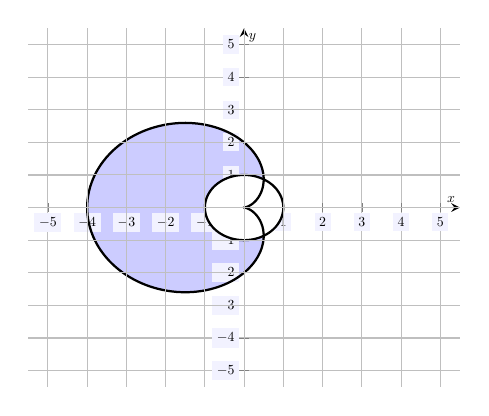
\begin{tikzpicture}[scale=0.8,every node/.style={scale=0.5}]
	\begin{axis}[
	grid=both,
	axis lines=middle,
	ticklabel style= {fill= blue!5!white},
	xmin= -5.5, xmax=5.5,
	ymin= -5.5, ymax=5.5,
	xtick= {-5,-4,...,5},
	ytick= {-5,-4,...,5},
	minor tick = {-5,-4,...,5},
	xlabel= \(x\), ylabel= \(y\)
	]
	\addplot[thick, samples=100, smooth, domain= -2*pi:2*pi,name path = circ,fill=white] ({cos(deg(x))},{sin(deg(x))});
	\addplot[thick, samples=100, smooth, domain= -2*pi:2*pi,name path = card,fill opacity=0.30] ({2*(1 - cos(deg(x)))*cos(deg(x))},{2*(1 - cos(deg(x)))*sin(deg(x))});
	\addplot[fill = blue!20] fill between [of=card and circ,soft clip = {domain=-2*pi:2*pi}];
	\draw[line width=0.015cm] (-5.5,0) -- (5.5,0);

	\pgfplotsinvokeforeach{-4,-3,...,1} {
	\draw[line width=0.012cm,lightgray] (#1,-5.5) -- (#1,5.5);
	}
	\pgfplotsinvokeforeach{-3,-2,...,3} {
	\draw[line width=0.012cm,lightgray] (-5.5,#1) -- (5.5,#1);
	}
	\end{axis}
	\end{tikzpicture}
	}
	\] \pspace

\sol{First, we find where the curves intersect:
	\[
	\begin{gathered}
	1= 2 - 2\cos \theta \\
	-1= -2 \cos \theta \\
	\cos \theta= \dfrac{1}{2} \\
	\theta= \dfrac{\pi}{3}, \; \dfrac{5\pi}{3}
	\end{gathered}
	\]
Let $A$ be the desired area. Let $A_1$ be the area bound by the circle $r= 1$ and the origin on $[\frac{\pi}{3}, \frac{5\pi}{3}]$ and let $A_2$ be the area bound by the cardioid $r= 2 - 2 \cos \theta$ and the origin on $[\frac{\pi}{3}, \frac{5\pi}{3}]$. We then know that $A= A_2 - A_1$. We need only compute these areas. Recall that area between a curve $r= r(\theta)$ and the origin is given by $\ds\frac{1}{2} \int_\alpha^\beta \big( r(\theta) \big)^2 \;d\theta$. First, we have\dots
	\[
	A_1= \dfrac{1}{2} \int_{\pi/3}^{5\pi/3} 1^2 \;d\theta= \dfrac{1}{2} \int_{\pi/3}^{5\pi/3} 1 \;d\theta= \dfrac{1}{2} \cdot \theta \bigg|_{\pi/3}^{5\pi/3}= \dfrac{1}{2} \left( \dfrac{5 \pi}{3} - \dfrac{\pi}{3} \right)= \dfrac{1}{2} \cdot \dfrac{4 \pi}{3}= \dfrac{2 \pi}{3}
	\]
As for $A_2$, we have\dots
	\[
	\begin{aligned}
	A_2&= \dfrac{1}{2} \int_{\pi/3}^{5\pi/3} (2 - 2 \cos\theta)^2 \;d\theta \\
	&= \dfrac{1}{2} \int_{\pi/3}^{5\pi/3} (4 - 8 \cos \theta + 4 \cos^2 \theta) \;d\theta \\
	&= \dfrac{1}{2} \int_{\pi/3}^{5\pi/3} 4 \;d\theta - \dfrac{1}{2} \int_{\pi/3}^{5\pi/3} 8 \cos \theta \;d\theta + \dfrac{1}{2} \int_{\pi/3}^{5\pi/3} 4 \cos^2 \theta \;d\theta \\
	&= 2 \int_{\pi/3}^{5\pi/3} 1 \;d\theta - 4 \int_{\pi/3}^{5\pi/3} \cos \theta \;d\theta + 2 \int_{\pi/3}^{5\pi/3} \cos^2 \theta \;d\theta
	\end{aligned}
	\]
We compute each of these integrals separately. The first two integrals are routine:}

\remove{\newpage

\sol{%
\thispagestyle{empty}
	\[
	\begin{aligned}
	2 \int_{\pi/3}^{5\pi/3} 1 \;d\theta&= 2 \cdot \theta \bigg|_{\pi/3}^{5\pi/3}= 2 \left( \dfrac{5 \pi}{3} - \dfrac{\pi}{3} \right)= 2 \cdot \dfrac{4 \pi}{3}= \dfrac{8 \pi}{3} \\[0.3cm]
	-4 \int_{\pi/3}^{5\pi/3} \cos \theta \;d\theta&= -4 \cdot \sin \theta \bigg|_{\pi/3}^{5\pi/3}= -4 \left( \sin(\tfrac{5\pi}{3}) - \sin(\tfrac{\pi}{3}) \right)= -4 \left( -\tfrac{\sqrt{3}}{2} - \tfrac{\sqrt{3}}{2} \right)= -4 \cdot -\sqrt{3}= 4 \sqrt{3}
	\end{aligned}
	\]
For the third integral, we use the identity $\cos^2 \theta= \dfrac{1 + \cos(2\theta)}{2}$:
	\[
	\begin{aligned}
	2 \int_{\pi/3}^{5\pi/3} \cos^2 \theta \;d\theta&= 2 \int_{\pi/3}^{5\pi/3} \dfrac{1 + \cos(2\theta)}{2} \;d\theta \\
	&= \int_{\pi/3}^{5\pi/3} (1 + \cos 2\theta) \;d\theta \\
	&= \theta + \dfrac{\sin 2 \theta}{2} \bigg|_{\pi/3}^{5\pi/3} \\
	&= \left( \dfrac{5 \pi}{3} + \dfrac{\sin \left(\tfrac{10 \pi}{3} \right)}{2} \right) - \left( \dfrac{\pi}{3} + \dfrac{\sin \left(\tfrac{2 \pi}{3} \right)}{2} \right) \\
	&= \left( \dfrac{5 \pi}{3} + \dfrac{-\tfrac{\sqrt{3}}{2}}{2} \right) - \left( \dfrac{\pi}{3} + \dfrac{\tfrac{\sqrt{3}}{2}}{2} \right) \\
	&= \left( \dfrac{5 \pi}{3} - \dfrac{\sqrt{3}}{4} \right) - \left( \dfrac{\pi}{3} + \dfrac{\sqrt{3}}{4} \right) \\
	&= \dfrac{5 \pi}{3} - \dfrac{\sqrt{3}}{4} - \dfrac{\pi}{3} - \dfrac{\sqrt{3}}{4} \\
	&= \dfrac{4 \pi}{3} - \dfrac{\sqrt{3}}{2}
	\end{aligned}
	\]
Therefore, we have\dots
	\[
	\begin{aligned}
	A_2&=  2 \int_{\pi/3}^{5\pi/3} 1 \;d\theta - 4 \int_{\pi/3}^{5\pi/3} \cos \theta \;d\theta + 2 \int_{\pi/3}^{5\pi/3} \cos^2 \theta \;d\theta \\
	&= \dfrac{8 \pi}{3} + 4 \sqrt{3} + \left( \dfrac{4 \pi}{3} - \dfrac{\sqrt{3}}{2} \right) \\
	&= 4 \pi + \dfrac{7 \sqrt{3}}{2}
	\end{aligned}
	\]
This shows that\dots
	\[
	A= A_2 - A_1= \left( 4 \pi + \dfrac{7 \sqrt{3}}{2} \right) - \dfrac{2 \pi}{3}= \dfrac{10 \pi}{3} + \dfrac{7 \sqrt{3}}{2}= \boxed{\dfrac{20 \pi + 21 \sqrt{3}}{6}}
	\]
\setcounter{page}{20}
   }
}



% Bonus II
\newpage
\noindent {\bfseries Bonus II.} Find a parametrization for the curves described below:
	\begin{enumerate}[(a)]
	\item A circle with radius 5 centered at $(-2, 3)$. \vfill
	\sol{%
		\[
		\begin{cases}
		x= 5 \cos(\theta) - 2 \\
		y= 5 \sin(\theta) + 3
		\end{cases}
		\qquad \text{ OR} \qquad \big( 5 \cos(\theta) - 2, 5 \sin(\theta) + 3 \big), \qquad\qquad \theta \in [0,2 \pi]
		\]
	} \vfill
	
	\item The line $y= 2x + 3$. \vfill
	\sol{%
		\[
		\begin{cases}
		x= t \\
		y= 2t + 3
		\end{cases}
		\qquad \text{ OR} \qquad \big( t, \; 2t + 3 \big), \qquad\qquad t \in (-\infty, \infty)
		\]
	} \vfill
	
	\item The portion of the parabola $x= y^2 - 3$ between $y= -1$ and $y= 2$. \vfill
	\sol{%
		\[
		\begin{cases}
		x= t^2 - 3 \\
		y= t
		\end{cases}
		\qquad \text{ OR} \qquad \big( t^2 - 3, \; t \big), \qquad\qquad -1 \leq t \leq 2
		\]
	} \vfill
	\end{enumerate}

\end{questions}
\end{document}